
\begin{figure}
   \centering
   \includegraphics[width=0.5\textwidth]{scheme.pdf}
   \usecaption{F_scheme} \label{F_scheme}
\end{figure}
 
\begin{figure*}
   \centering
   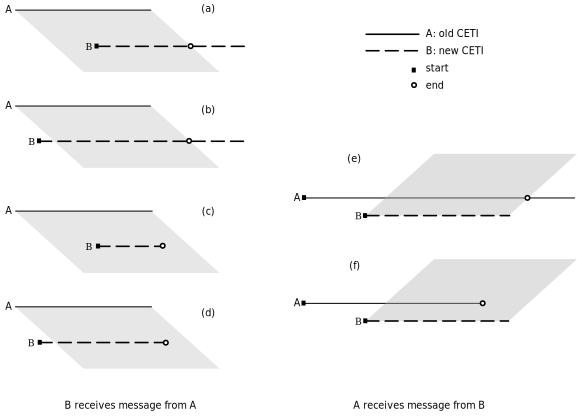
\includegraphics[width=0.8\textwidth]{Messages_01.pdf}
   \usecaption{F_messages} \label{F_messages}
\end{figure*}
      

%%% S E C T I O N - - - - - - - - - - - - - - - - - - - - - - -
\section{Methods and working hypotheses}\label{S_methods}
%{{{

Simulations are suitable tools to analyze systems that evolve with
time and involve randomness.
%
An advantage of simulations compared to theoretical approaches, is
that the former usually require less assumptions and simplifications,
and can be applied to systems where a theoretical model can not be
found.
%
In particular, many complex stochastic processes that can be described
by the evolution of the state of a system, can be efficiently modeled
with the discrete--event (hereafter, DE) simulation approach.
%
A system described with the DE paradigm is characterized by a set of
actors and events, where actors interact causally through a series of
events on a timeline and process these events in chronological order
\citep{ptolemaeus_system_2014, chung_simulation_2003,
ross_simulation_2012}.
%
Each event produces changes in the values of the variables that define
the process, and thus the corresponding change in the state of the
simulated system.
%
This method is well suited for the particular case of the diffusion of
intelligent signals in the Galaxy, and allows to explore several
models easily.
%
We simulate the statistical properties of a set of points in space and
time that have a causal connection
at light speed, hereafter dubbed ''causal contact nodes'' (\ceti).
%
% ability of emitting and receiving messages at
%
We chose this generic name in order to stress the fact that in this
analysis no broadcasting or lookout activities are required, 
and therefore not actual messages are considered, only the causal
contact.
%
For the special case of a fully efficient node that emits
and receives isotropically, a causal contact node can be considered as
a broadcasting station that has the ability to detect signals through
an active lookout program.
%
Also, it is worth mentioning that this is a general approach, and not
necessarily a \ceti is the host of an intelligent civilization.
%
It can be associated with a planet where life has developed,
became intelligent, reached the skills required to find the right
communication channel, sustain a search and establish a contact.
%
Alternative message processing entities could be considered, for
example interstellar beacons where life has ceased to exist but
continue with its emission or communication stations established by
probes or left intentionally by intelligent beings \citep[see, e.g.,
][]{peters_outer_2018, barlow_galactic_2013}.
%
In principle, these strategies could affect our results since it would
be easier to configure a cluster of \cetis that spread in time.
%
However, we do not consider this highly speculative alternatives at
this point.
%
% have been proposed
%
For the purpose of this analysis, only the communication capability is
relevant, since we study the causal contacts between the locations.
%
The system is defined by a number of actors that represent \cetis and
appear at different instants in time, generating events that produce
meaningful changes in the variables that describe the system, i.e., in
the arrangement of \cetis and their network of causal contacts.
%
For example, the appearance of a new \ceti in a region which is filled
with a signal emitted by another \ceti, will increase the number of
active \cetis and the number of pairs of \cetis in causal contact.
%
Assuming some simple hypotheses, the discrete events method can be
performed taking into account a small number of variables, which allow
to analyze the variation of the results in the model parameter space.


In what follows, we describe the experimental setup chosen to estimate
the probabilities of causal contacts and several derived quantities in
terms of three independent parameters, namely, the mean time span
between the appeareance of consecutive \cetis, ($<\tau_a>$), their mean
lifetime ($<\tau_s>$), and the maximum distance a signal can be
detected by another \ceti ($D_{max}$).
%
Intuitively, the shorter the $\tau_a$ parameter and the larger the
$\tau_s$ and $D_{max}$ parameters are, the greater the probability of
the existence of causal contacts between pairs of \cetis would be.
%
We also need to propose theoretical distribution functions for both
the distribution of lifespans ($\tau_s$) and the distribution of the
number of \cetis per unit time \citep{maccone_evolution_2014,
Sotos_biotechnology_2019}, related to the time span between the
appeareance of consecutive \cetis (since when $<\tau_a>$ is shorter, it
produces a greater density of \cetis).
%
The shapes of these distributions are set to a fixed law, as discussed
in Sec.~\ref{SS_PDF_shape}.


A causal connection can be produced without the need of the two
involved locations being concurrent or active at the same time.
%
This is a fundamental property of the system which arises as a
consequence of the large spatial and temporal scales, where a message
is transmitted at light speed.
%
Although a \ceti could be active for enough time so as to transmit a
message at large distances, the limited power of the message and the
dilution that runs as the squared distance from the source, imposes a
detectability limit.
%
As a consecuence of this limitation and of their finite lifetime,
considered as the period of time between the acquisition and loss of
communicating capacity, each \ceti will fill a spherical shell region of
the Galaxy, limited by two concentric spherical surfaces.
%
The leading front, or surface of first contact (SFC) grows from the
central \ceti until it reaches the maximum distance $D_{max}$.
%
Thus, the volume reached causally by a \ceti is initially a growing
sphere.
%
Following the end of the civilization, there is still a region which
is filled with the emitted signals.
%
The trailing front, or surface of last contact (SLC) also grows from
the central \ceti, with a delay with respect to the SFC equivalent to
the lifetime of the \ceti, and produces a spherical shell region.
%
Any other \ceti within this region will be aware of the originating
\ceti,
even if it has disappeared before the time of contact.
%
This region will grow if the surface of first contact has not yet
reached the maximum distance $D_{max}$, and will shrink otherwise
until the surface of last contact reaches $D_{max}$, producing as a
result the loss of all signal from the central \ceti.
%
In our approach, we consider a model Galaxy where the width of the
disk is negligible with respect to the radius of the disk, so that the
\cetis are placed on a 2D plane disk.
%
In the 2D simulation only the intersection of the communicating
spherical shells with the plane of the galaxy is relevant, and produce
the corresponding circles or rings for the filled spheres or annular
regions of the spherical shells, respectively.
%
We illustrate in the Fig.~\ref{F_scheme} the schematic representation
of the region causally connected to the central \ceti.
%
To this end, we use space--time diagrams, where time is represented on
the horizontal axis, and space is represented in the vertical axis.
%
A growing surface of first contact in this diagram is represented as a
growing circle, centered on a point in the time axis, which shifts
towards the right at the same rate the radius of the circle increases.
%
The maximum distance of the message limits the radius of the circles,
so that once this distance is reached, the circle continues its shift
towards the right, but maintaining a constant radius.
%
At the end of the lifetime of a \ceti, a growing surface of last
contact is represented by a circle that covers the inner part of the
causal region, producing a ring of diminishing area (panel (a)).
%
In this scheme, the entire lifetime of a \ceti can then be represented
by a polygon, limited in the spatial axis by the maximum distance of
the signal $D_{max}$ and in the time axis by the time span between the
starting time (concave vertex) and the ending time (convex vertex).
%
This representation allows to easily visualize the important events
that result from the existence and communications of two \cetis (panel
(b)).
%
The points in time where the \cetis acquire their communicating capacity
(CC) are dubbed ''awakening'' events ($A_1$ and $A_2$ in the Figure).
%
Similarly, the points in time where the \cetis loss their
communicating capacity are dubbed ''doomsday'' events ($D_1$ and $D_2$
in the Figure).
%
The points in space--time where the first contact is produced for each
one of the \cetis, are defined as ''contact'' events, shown as $C_1$
and $C_2$ in the Figure.
%
Finally, the two points where the contact is lost for each one the
\cetis, are denominated ''blackout'' events, shown as $B_1$ and $B_2$
in the Figure.
%
It is important to notice that there is a time delay between the
contact events of the two \cetis involved in this analysis, and also a
time delay between the two blackout events, so that the time range
when a bidirectional contact is possible occurs between the maximum
time of the contact points and the minimum time between the blackout
points.




The initially growing communicating sphere, is shown over
space--time diagrams, where time is represented on the horizontal
direction, and space is represented in the vertical direction.
%
In the upper panel (a), the sphere is growing as the surface of first
contact has not reached the maximum distance.
%
In the middle panel (b) it has reached the maximum distance, so that
it remains at the same size.
%
After a Doomsday event (bottom panel, b), the signals can still be
observed, but the surface of last contact grows.
%
We also show in this Figure a schematic representation of two
emitters, E$_1$ and E$_2$, that reach each other at different times.
%
The time span for E$_i$ is (A$_i$ , D$_i$) , for $i = {1, 2}$.
%
Emitter $i$ can listen to emitter $j$ between C$_{ij}$ and B$_{ij}$.
%
The type and length of causal contact in both directions depend on the
distance and time lag between the awakening events, the maximum
distance that a signal can reach and the time period in which each
emitter is active.
%
In the Fig.~\ref{F_messages} we show a schematic representation of the
possible cases in which a \ceti A can be in causal contact with a
\ceti
B which appears later.
%
The duration of the causal contact in one direction depends on several
factors, mainly $\Delta$t~A , $\Delta$t~C , and $\Delta$X.


The temporal structure of the process is defined by two distribution
parameters that represent the mean time interval that an intelligent
civilization can emit and receive signals, and the mean time interval
between the emergence of an intelligent communicating civilization and
the next one.
%
The spatial structure of the simulation is given by the size and shape
of the Galactic Habitable Zone and the maximum distance a signal can
travel to be detected.
%
The parameters for the temporal distributions also determine the
spatial properties since the density of active \cetis in the Galaxy
depend on these two parameters.
%
For example, a small $\tau_a$ and a large $\tau_s$ will produce a
Galaxy densely populated with \cetis, and vice versa.
%
Also, some hypotheses must be made in order to complete the
simulation.
%
\citet{forgan_spatiotemporal_2011} argues that the times at which
different civilizations become intelligent follow a Gaussian
distribution, and then the distribution of inter-arrival times is an
inverse exponential.
%
We chose to assume that the distribution of the times of A events is a
stationary Poisson process, and then the distribution of the times
between the appeareance of new consecutive \cetis is exponential.
%
Regarding the duration of a \ceti, we propose that the distribution of
the duration of \cetis is a stationary exponential distribution.
%
\citet{balbi_impact_2018} stress the fact that it would be desirable
to arrive at a theoretical statistical distribution of the lifespan of
civilizations, preferentially on the basis of the underlying
astrophysical and biological processes.
%
\citet{maccone_lognormals_2014} argues that this distribution should
be a log normal.  (EXPAND)



There is no a temporal window for the model, i.e., the simulation
starts when the process is already stable, and ends before any
galactic effect could modify or affect of fixed variables.
%
The probability for the rise of a \ceti is homogeneous over the GHZ.
%
Although the Galaxy has a well known spiral structure, the assumed
sparsity of civilizations makes this assumption very reasonably.
%
Otherwise, if the distribution of civilizations is not sparse, it
could be the case that the spiral arms would host most of the
civilizations, and contacts are frequent between closely located
civilizations.
%
In such a case we could expect that the interpretation of our results
could be considered as pessimist for the establishment of a contact with
our planet.
%
We also limit the posibilities of life or other types of civilizations
to the hypothesis usually stated for the definition of the GHZ
\citep{dayal_habitability_2016, gonzalez_galactic_2001,
lineweaver_galactic_2004, gonzalez_habitable_2005,
morrison_extending_2015, haqq-misra_evolution_2019,
rahvar_cosmic_2016, gobat_evolution_2016, rahvar_cosmic_2016}.
%
\citet{vukotic_astrobiological_2012} propose probabilistic cellular
automata model to explain the astrobiological history of the Milky
Way.
%
This means that we set aside possible civilizations that could survive
in severe conditions or unstable systems, which would prevent the
appeareance of life as we know it.


While the aforementioned assumptions are basic conditions for most of
the stochastic processes observed in nature, we need to make stronger
assumptions related to the nature of the message.
%
The most simple assumption about the message itself, is that it
travels at light speed.
%
With this, we are considering messages sent through, for example,
electromagnetic radiation or even gravitational radiation, but we set
apart messages sent with mechanical means or physical objects, or
through some unknown technology that violates the known so far laws of
physics.
% 
For the communication of \cetis through messages sent isotropically, we
assume that the capacity to emit signals and to receive signals occur
at the same time.
%
This means that the ability to find another civilization develops at
the same time that the ability and intention to emit a signal in all
direction, intended to be detected by an unknown civilization.
%
Although there are several reasons to think that this could not be the
case, at large time scales it can be considered that both abilities
occur roughly at coincident epochs.
%
Another essential assumption is that all \cetis use the same signal
power, so that there is a maximum distance out to which it can be
detected.
%
It is worth mentioning that we are considering in our experimental
setup a system composed by several emiters and receivers across the
Galaxy, under the hypothesis proposed before.
%
In such a system we compute probabilities of a \ceti making contact
with another \ceti, and the results must be interpreted as for a
randomly chosen \ceti, given certain conditions of homogeneity on an
ensemble of equivalent galaxies.
%
We stress the fact that we are not centered on the probabilities for
the Earth itself, but on a generalized \ceti.
%
Regarding the extent of the signals, we know that the distance from
which a signal from Earth could be detected using the current
technology is of a few hundreds light years, given that the signal was
sent to a specific direction.

               

%https://setiathome.berkeley.edu/forum_thread.php?id=80585&postid=1833000#1833000]
%https://www.engadget.com/2017/05/25/listening-to-starlight-our-ongoing-search-for-alien-intelligenc/]
%[from https://en.wikipedia.org/wiki/Fermi_paradox]
%
It is straightforward to propose and implement a distribution of
maximum distances, although this would increase the model complexity
at the cost of a larger uncertainty or of another dimension on the
hypothesis space.
%
This proposal is based on a pronoid scenario (REF), and we do not
consider in this work the occurrence of paranoid or partially paranoid
civilizations.
%
If that would be the case, the results obtained here can be taken as
upper limits.



In our simulations we also assume the simplest situations for the
growth of the sphere of first contact.
%
For example, we discard the possibility of stellar colonization
\citep[e.g.][]{newman_galactic_1981, walters_interstellar_1980,
starling_virulence_2013, barlow_galactic_2012, jeong_large_2000,
maccone_mathematical_2011} and assume that the communication aim is
performed to all directions with the same power and the same
probability, i.e., strongly assume isotropic communication in all
cases.
%
More detailed simulations could be produced considering different
efficiency of communication or detection methods.
%
%Also, a mixed paranoid/pronoid population of intelligent civilizations
%could be implemented easily.
%
% EXPLICARLO O SACARLO
% O PONER EN LA DISCUSION
%
However, in this case we also would complicate the experimental setup,
make the results less evident.
%
The results are independent of the nature of life (organic or
artificial).
%
The lifetime of a civilization can be caused by auto destruction or by
external factors.
%}}}


\subsection{Power laws vs. exponential laws}\label{SS_PDF_shape}
%{{{

The exponential distribution of lifespan and waiting times is
justified by considering that the process of appeareance of life in
the galaxy is homogeneous and stationary.
%
Equivalently there is no preferred location within the GHZ for the
spontaneous appeareance of life, and that the emergence of a
civilization is independent of the existence of previous civilizations
in the galaxy.
%            
This is equivalent to proposing a Poisson process for the emergence of
\cetis, since there is a close relation between the number of events in
time or space and the waiting time or separation, respectively.
%
That is, these are two alternative approaches to describing the same
process, a Poisson distribution for the number of events implies an
exponential distribution for their separations, and viceversa.
%
It should be emphasized that the exponential laws used in this work
are assumed, although instead of analyzing results from a particular
parameter chosen ad--hoc, we explore the hypothesis space and analyze
the impact of the values of these parameters on the results.
                                                           

The power law and exponential statistical distributions are among the
most common patterns found in natural phenomena.
%
For example, the distribution of the frequency of words in many
languages is known to follow a Zipf law (which is a power law).
%
Zipf law also describes population ranks of cities in various
countries, corporation sizes, income rankings, ranks of number of
people watching the same TV channel (Zipf's law).
%
% CITAR ALGO DE LA LEY DE ZIPF
%
The magnitudes of earthquakes, hurricanes, volcanic eruptions and
floods; the sizes of meteorites or the losses caused by business
interruptions from accidents, are also well described by power laws
(Sornette 2006).
%
The power law behaviour has been observed in a variety of systems,
including for example stock market fluctuations, sizes of computer
files and word frequency in languages \citep{mitzenmacher_brief_2004,
newman_power_2005, simkin_theory_2006}
%
Power laws have also been widely used in biological sciences, e.g., in
analyzing connectivity patterns in metabolic networks
\citep{jeong_large_2000} and in the number of species observed per
unit area in ecology \citep{martin_origin_2006, frank_common_2009}.
% 
More examples can be found in the literature
\citep{martin_origin_2006, maccone_KLT_2010, barabasi_scale_2009,
maccone_evolution_2014, maccone_lognormals_2014,
benguigui_classificacion_2016}
 
%}}}

\subsection{Discrete event process}
%{{{

Given a parametric model $M(\tau_a, \tau_s, D_{max})$, which includes
the functional forms of the statistical distributions and fixed values
for the hypotheses, a discrete event simulation is performed by
keeping track of a set of variables that change each time a meaningful
event is produced.
%
The main variables that follow the evolution of the simulation are the
positions of stars, which are sampled randomly within the GHZ, the
time of the awakening of each \ceti (A event), and the time of the
vanishing of each \ceti (D event).
%
The variables that can be deduced from the previous ones include the
number of \cetis in casual contact with at least another \ceti at a given
time, the number of \cetis as a function of time, the number of \cetis
that receive a message at least one time, the number of \cetis that
receive a message at least one time and successfully deliver an answer
and the number distribution of waiting time to receive a message.
%
All these quantities are updated each time one of the four events (A,
B, C, D) is produced.
          
%%% comparar con el stochsatic cellular automata
% ver libro Solving Fermi paradox, sec. 27.3.1

%}}}

           
\begin{figure} \centering
   \includegraphics[width=0.5\textwidth]{F1.pdf}
   \usecaption{F_number_of_contacts} \label{F_number_of_contacts}
\end{figure}
        

\subsection{Model for \cetis}
%{{{

Since the method is based on events, the first step is to define an
architecture of events, the relationships between them and how events
trigger changes on the state of the system.
%
We consider a simulated system that represents the galactic habitable
zone (GHZ).
%
On a first approach, the GHZ is a 2-dimensional annular region.
%
The adopted values for the GHZ are 20 kly and 60 kly, for the inner
and outer radius, respectively \citep{lineweaver_galactic_2004}.
% ojo, ese paper dice 7-9 kpc, o sea tiene un limite superior mucho
% mas chico...
%
This simple model does not take into account the variations in stellar
density given by the spiral structure.
%
Although there are several possible approaches, we chose to follow the
evolution of the system according to the following events:

\begin{enumerate}
   \item[(A)] Awakening: A new \ceti acquires the ability to emit
      and receive messages and starts to actively broadcast and
      lookout for messages.
   \item[(C)] Contact: A new one-way causal contact is established
      (does not require the awareness of the involved \cetis.)
   \item[(B)] Blackout: An existing causal contact is interrupted,
      with or without the occurrence of a doomsday event.
   \item[(D)] Doomsday: An old \ceti disappears, or halts its
      communication activities.
\end{enumerate}

We have chosen this nomenclature so that it can be easily remembered
from the initial A, B, C, D.
%
The \blackout is produced when one of the two \cetis halts in its
capability of emiting and receiving signals.
%
It can occur at the same time the \doomsday or before.
%
Similarly, a \ccontact can be produced at the time of the \aawakening
or later, and there can be several \contacts for the same \ceti.

                        

The system is updated each time an event is produced.
%
The time marks for each event (A and D for each \ceti and C and B for
each causal contact) are stored as a result of the simulation.
%
Also, the list of active \cetis is obtained as a function of time.
%
Some fixed variables must be set in order to carry out the simulation:
the size of the Galactic Habitable Zone, the mean lifetime of a \ceti,
$\tau_s$, the mean waiting time for the appeareance of another \ceti,
$\tau_a$, and the maximum distance a message can be detected.



The Galactic Habitable Zone is the only one of the four parameters
that is barely known, is set at fixed values of the inner and outer
radii, radial symmetry is assumed, and the with of the galactic disk is
neglected compared to the radial size.
%
The two radii are measured in light years, with the aim to maintain a
single and comprehensive unit for both space and time coordinates. 

The simulation was implemented on a python 3 code, which is publicly
available\footnote{https://github.com/mlares/simu\_contact}

%}}}
